\chapter{Implementação do Projeto}

\section{Bloco 0 - Conversão A/D no MSP430}
	
	\subsection{Análise de \textit{Hardware}}
	
		Antes do sinal chegar ao microcontrolador para o correto processamento do sinal de áudio, será necessário, conforme já relatamos, amostrar esse sinal através de valores corretamente quantizados. Para isso, conforme abordado na seção \ref{secao-conv-analogica-digital} deste trabalho, é necessário utilizar um Conversor Analógico Digital - ADC.
		
		O modelo do MSP 430 em questão (MSP430F5529LP) possui um ADC interno de 12 (doze) bits (ADC12). Ou seja, é possível representar em níveis de pulso até 4096 níveis. Algumas características podemos listar pois será objeto de avaliação dentro do projeto \cite{Davies2008}.
		
		\begin{itemize}
			\item Resolução de 12 bits monotônica, sem perdas de código;
			\item Velocidade nominal de até 200.000 amostras por segundo (200 Ksps), utilizando a técnica de aproximação sucessivas (SAR);
			\item Operação de com diversas referências internas de tensões: 1.5V, 2.0V, ou 2.5V com consumo típico de aproximadamente $250\mu A$ quando em operação;
			\item Canais de entrada exclusivos para sensor de temperatura interno, tensão de alimentação e tensões de referências externas;
			\item 16 memórias de conversão com controle independente de cada uma, inclusive com a capacidade de especificar o canal de entrada e referência;
			\item Fonte de \textit{clock} selecionáveis por softwares;
		\end{itemize}
	
		O coração de funcionamento desse módulo do microcontrolador consiste basicamente no seguinte:
		
			\begin{enumerate}[(i)]
				\item O processador usa dois níveis de tensões selecionáveis: $V_{R^{+}} $ e $ V_{R^{-}} $ afim de determinar o valor mínimo e máximo do conversor;
				\item Uma saída digital ($ N_{ADC} $) é setado no nível máximo ($ 4095 = 0FFFh $) quando o valor de entrada for igual ou até mesmo maior que $ V_R^+ $. De modo semelhante o valor digital ($ N_{ADC} $) será zero quando o valor de entrada for igual ou menor que $ V_{R^-} $.
				\item A equação básica da conversão é:
				
				\begin{equation}
					\label{eq-adc12-formula}
					N_{ADC} = 4095.\frac{V_{in}-V_R^-}{V_R^+ - V_R^-}
					\qquad
					V_{in}: \text{Tensão de entrada}.
				\end{equation}
				\item Em especial, o módulo ADC12\_A é configurado por dois registros de controle: o ADC12CTL0 e ADC12CTL1.
				\item  O modo de funcionamento do conversor (conversão simples ou sequência de canais) pode ser configurado pelos \textit{bits} CONSEQx (registrador ADC12CTL1);
				\item Após isso, seleciona-se o endereço inicial da memória de conversão, pelos \textit{bits} CSTARTADDx (registrador ADC12CTL1);
				\item Por fim, liga-se o conversor (\textit{bit} ADC12CTL0:ADC12ON=1) e habilitam-se as conversões (\textit{bit} ADC12CTL0:ENC=1).7
			\end{enumerate}
	
	\subsection{Requisitos de Hardware para a Tempo de Amostragem}
		
		\subsubsection{Contextualização}
		
		Um ponto importante a ser considerado, quando convertemos um sinal analógico qualquer numa sequência de valores digitais, é a precisão que estes valores representam o sinal original. 
		
		É claro que, na prática, é conveniente, para a escolha da taxa de amostragem, usar frequências muito maiores do que 2 vezes a do sinal e isso ocorre, por exemplo, quando possível.  Como é o caso  de sinais de áudio, especialmente em  CDs players,  em  que  a frequência de amostragem é de $44,1$ kbytes por segundo onde o que nos leva a 2 vezes a frequência máxima que podemos ouvir que é de 20 kHz.
		
		Por outro lado, o microcontrolador, em especial para a aplicação ora pretendida, são equipamentos alimentados por bateria e o consumo do dispositivo, nesse caso, é um requisito muito importante. Como a complexidade na obtenção das amostras aumenta em função da quantidade de amostragem que pode fazer e a potencialidade do microprocessador usado, é extremamente importante a escolha viável de uma taxa de amostragem (figura \ref{fig-taxa-de-amostragem-exemplos}) que atendam aos requisitos do projeto, ponderados com as limitações do equipamento em questão \cite{Braga2012}.
		
		\begin{figure}[!ht]
			\label{fig-taxa-de-amostragem-exemplos}
			\centering
			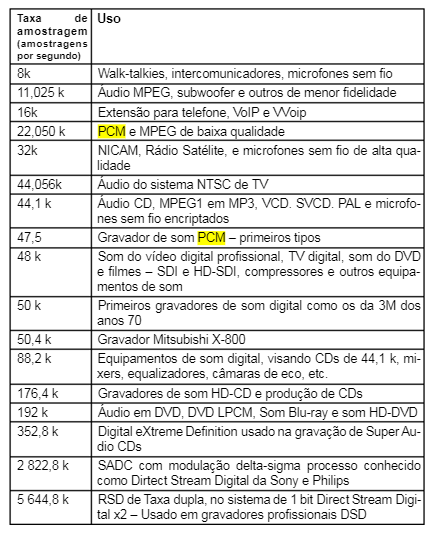
\includegraphics[scale=0.8]{./figuras/fig-exemplo-taxa-amostragem.png}
			\caption{Algumas taxas de amostragem utilizadas na prática}
		\end{figure}
	
		\subsubsection{Tempo de Amostragem do ADC12 do $\mu C$ MSP430}
			
			O conversor ADC do $\mu C$ aguarda a ocorrência de um sinal de disparo de conversão (SAMPCON) que pode ser originado de uma das quatro fontes\footnote{SHS\_1 por exemplo é proveniente da interrupção de um evento de comparação em um dos canais do timer A (saída TA1).} selecionadas pelos bits SHSx (registrador ADC12CTL1). Quando SAMCOMP = 0, todas as entradas analógicas ficam em alta impedância, caso contrário (SAMCOMP = 1), uma entrada Ax pode ser modelada como um circuito $RC$, passa baixa, durante o tempo de amostragem da conversão ($t_{sample}$).
			
			Uma equação, conforme o Guia do Usuário da Família de Microcontroladores MSP430x5xx, pode ser usada para cálculo do valor mínimo da taxa de amostragem para uma conversão de n-bits, no qual $ n $ é igual a quantidade de bits de resolução do conversor.
			
			\begin{equation}
				t_{sample} > (R_s + R_i) . \ln(2^{n+1}). C_i + 800ns
				\label{eq-circ-RC-msp430}
			\end{equation}
			
			A equação \ref{eq-circ-RC-msp430}  é oriunda de uma análise de um circuido \textit{RC} em descarregamento cuja resposta no domínio do tempo da tensão de saída é dada por:
			
			\begin{equation*}
				V_{out} = V_{in}e^{-t/{RC}}
			\end{equation*}
			
			Temos no caso, para uma quantização dos valores de tensão de entrada valores que podemos mensura-los em MSB e LSB. Considerando o caso mais simples onde a tensão de entrada estaria entre um bit 0 e 1 de uma quantização com apenas n byte ($ 2^n $ LSB`s) obtemos:
			
			\begin{equation}
				\begin{aligned}
						&\frac{V_f}{V_i} = e^{-t/{RC}}\Rightarrow \ln\left(\frac{V_f}{V_i}\right) = -\frac{t}{RC}\\
					&\ln\left(\frac{\frac{1}{2}LSB}{2^n LSB}\right) = -\frac{t}{RC}\Rightarrow \boxed{t = RC.\ln(2^{n+1})}
				\end{aligned}
			\end{equation}

			
			Por conseguinte, com SHP = 1 temos o modo de amostragem temporizada. O tempo de amostragem será determinado por um \textit{timer} interno, que é configurado de acordo com os bits SHT1x e SHT0x (registrador ADC12CTL0). Os \textit{bits} SHT1x determinam o tempo de amostragem (em ciclos de clock do conversor) para as memórias ADC12MEM8 até ADC12MEM15, tal como os \textit{bits} SHT0x determinam o tempo de amostragem para as memórias ADC12MEM0 até ADC12MEM7.
			
			Em suma, calculado o tempo de amostragem 
		
		
		
		
	
\section{Bloco 1 - Projetando um Filtro FIR}
	\subsection{Comunicação Serial}
		
\section{Bloco 2 - Implementando o \textit{Pitch-Shifter}}

\section{Bloco 3 - Delay Time}